\newpage
\section{Analog Watch}
\subsection{PCB}
After the PCBs for the BCD Version were working, i also created an analog Version, so i dont have to explain the Clock everytime ;-)

The Analog Watch features the same Schematics for the basic clock functionality, but the display is done via Charlieplexing the LEDs. There are 4 Clustes with 4 Pins which drive all the 42 LEDs. 12 LEDs on the inner ring are displaying the hours. On the outer ring 30 LEDs display the Minutes. Since it was not possible to fit 60 LEDs on the outer ring, uneven numbers are shown while lighting up the two neighbouring LEDs.
\begin{center}
  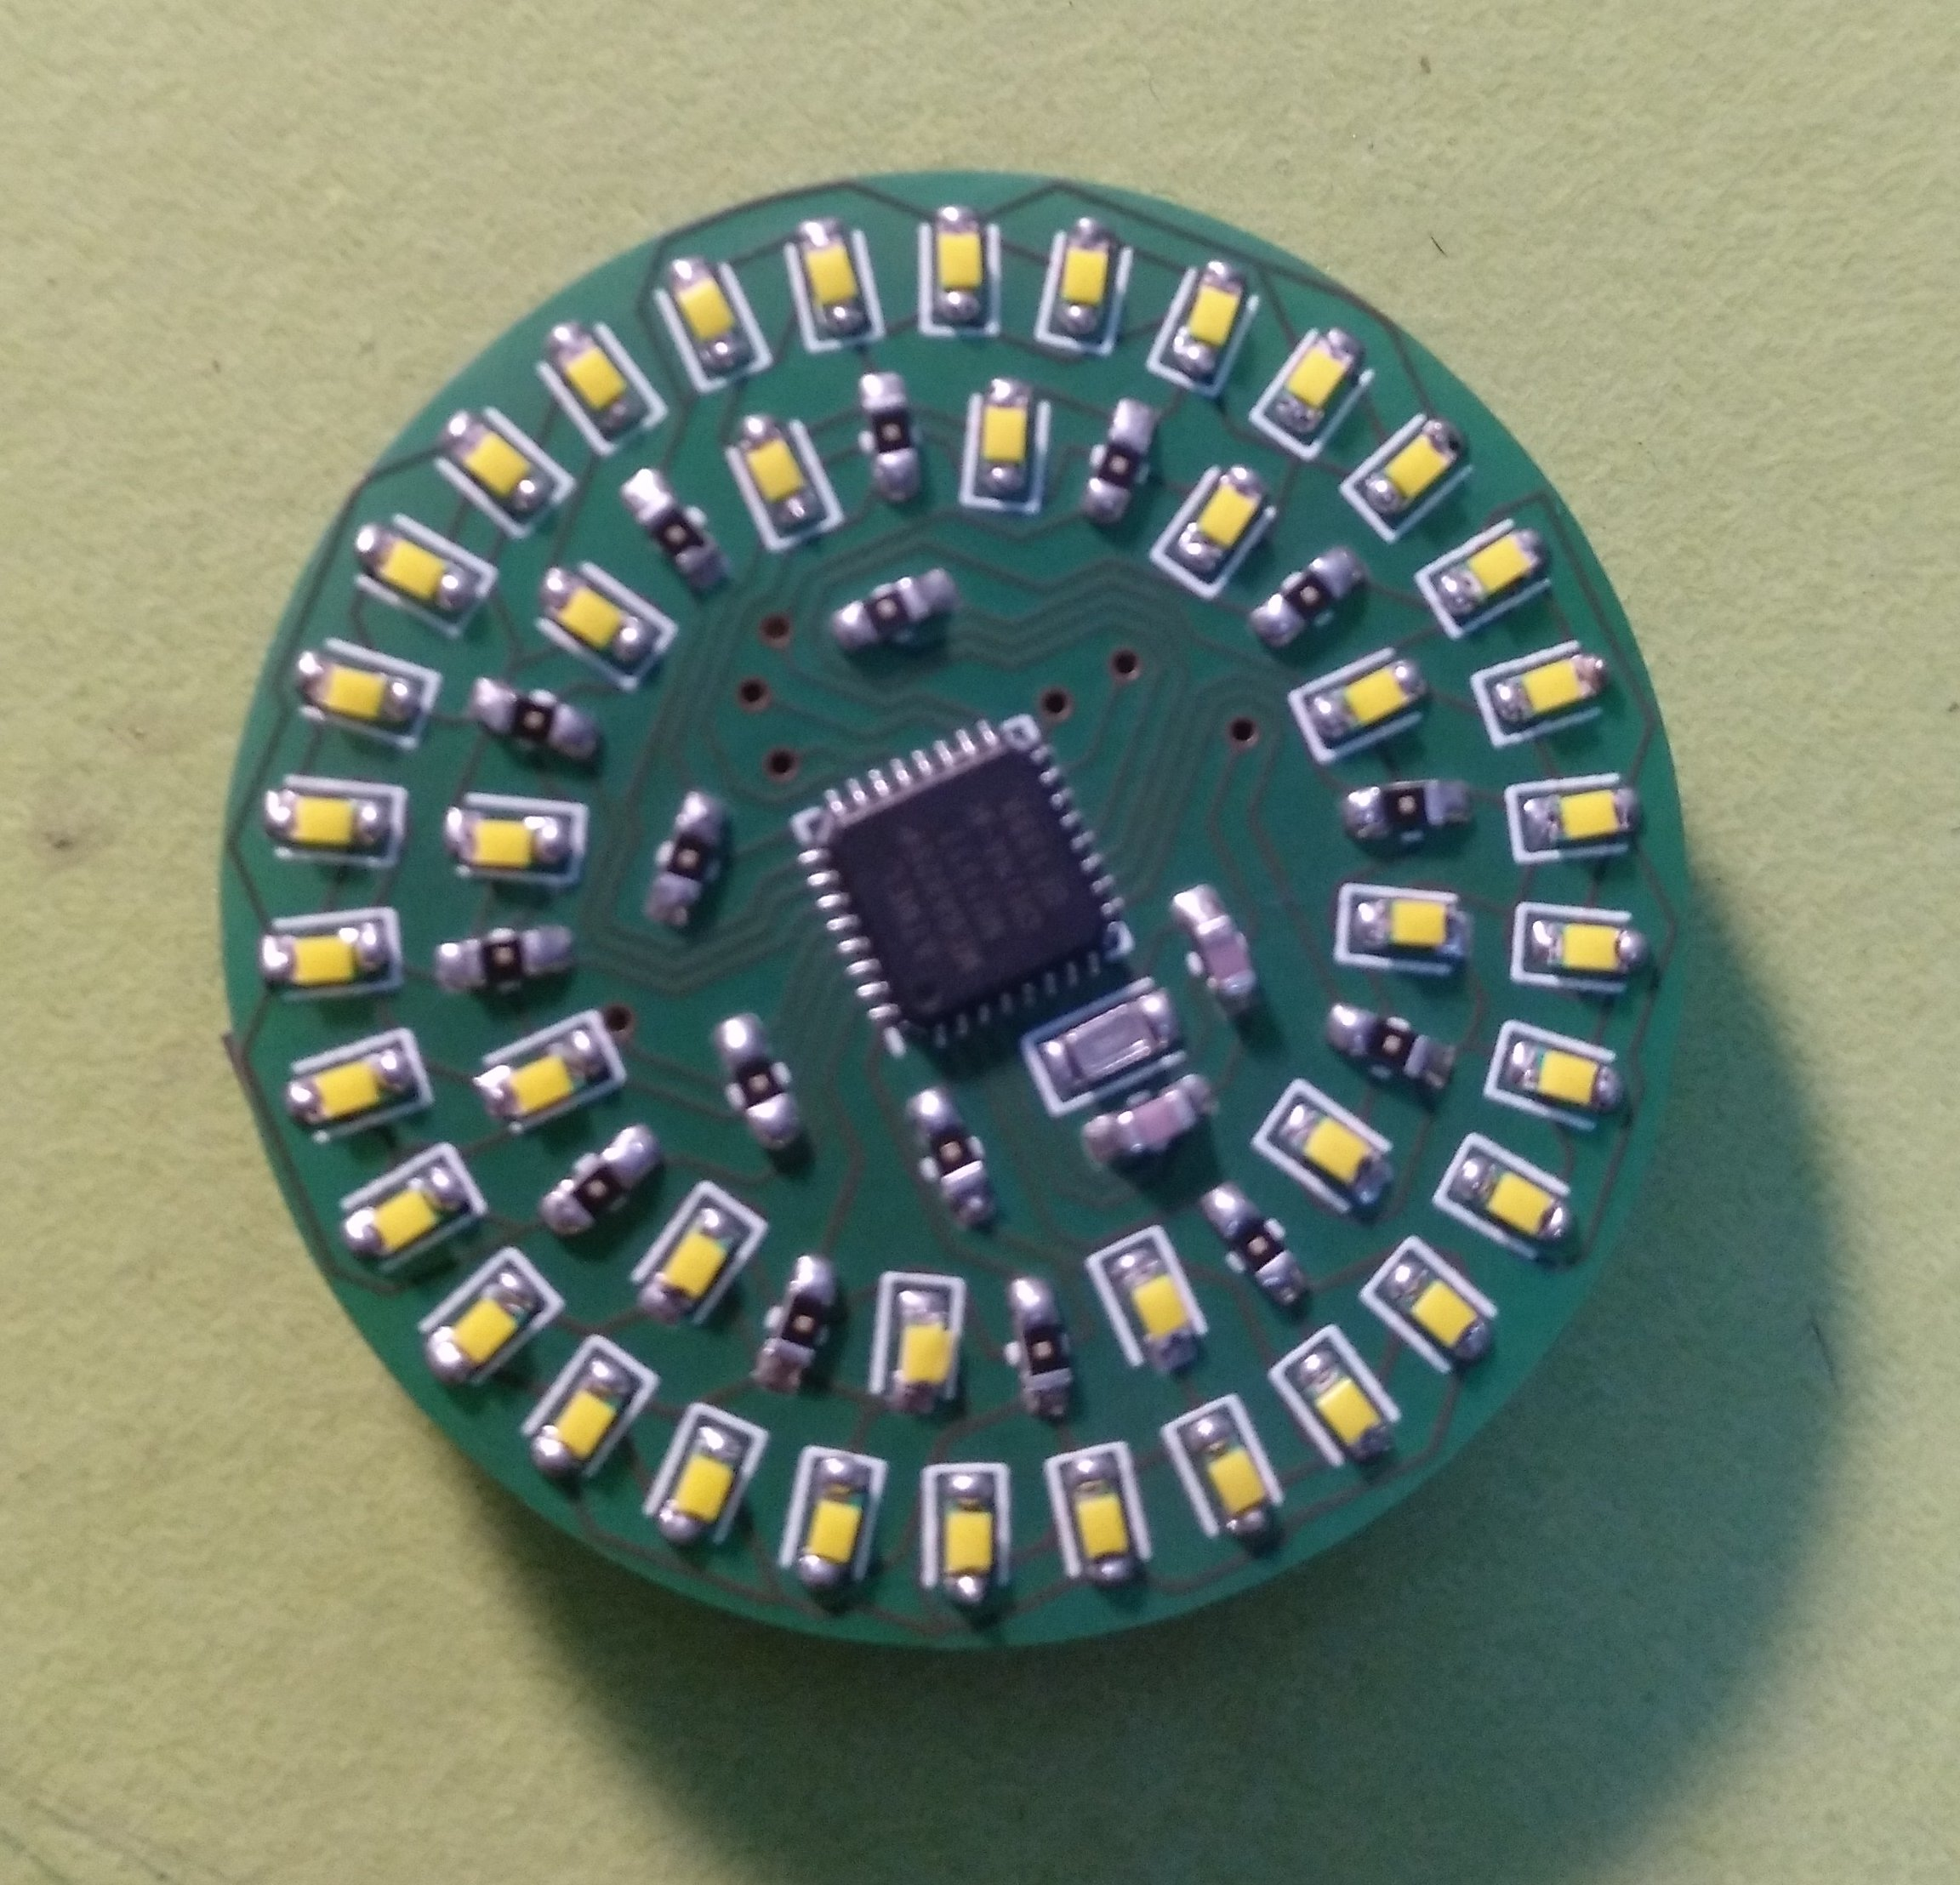
\includegraphics[width=0.5\textwidth]{../Pictures/AnalogPCB.jpg}
\end{center}
\newpage

\subsection{Housing}
The PCB for the analog Version is designed with the same mechanical Interface as the Binary Version therefore the Housing from the Binary Version can be used.

\subsection{first Watch which i gave away}
The first Watch i gave away was one of the analog PCB ones i built for my dads birthday.
for this Watch i replaced all the resistors for the LEDs with Zero $\Omega$ resistors, so the LEDs got more bright and are clearly readable also in the sunlight.
\begin{center}
  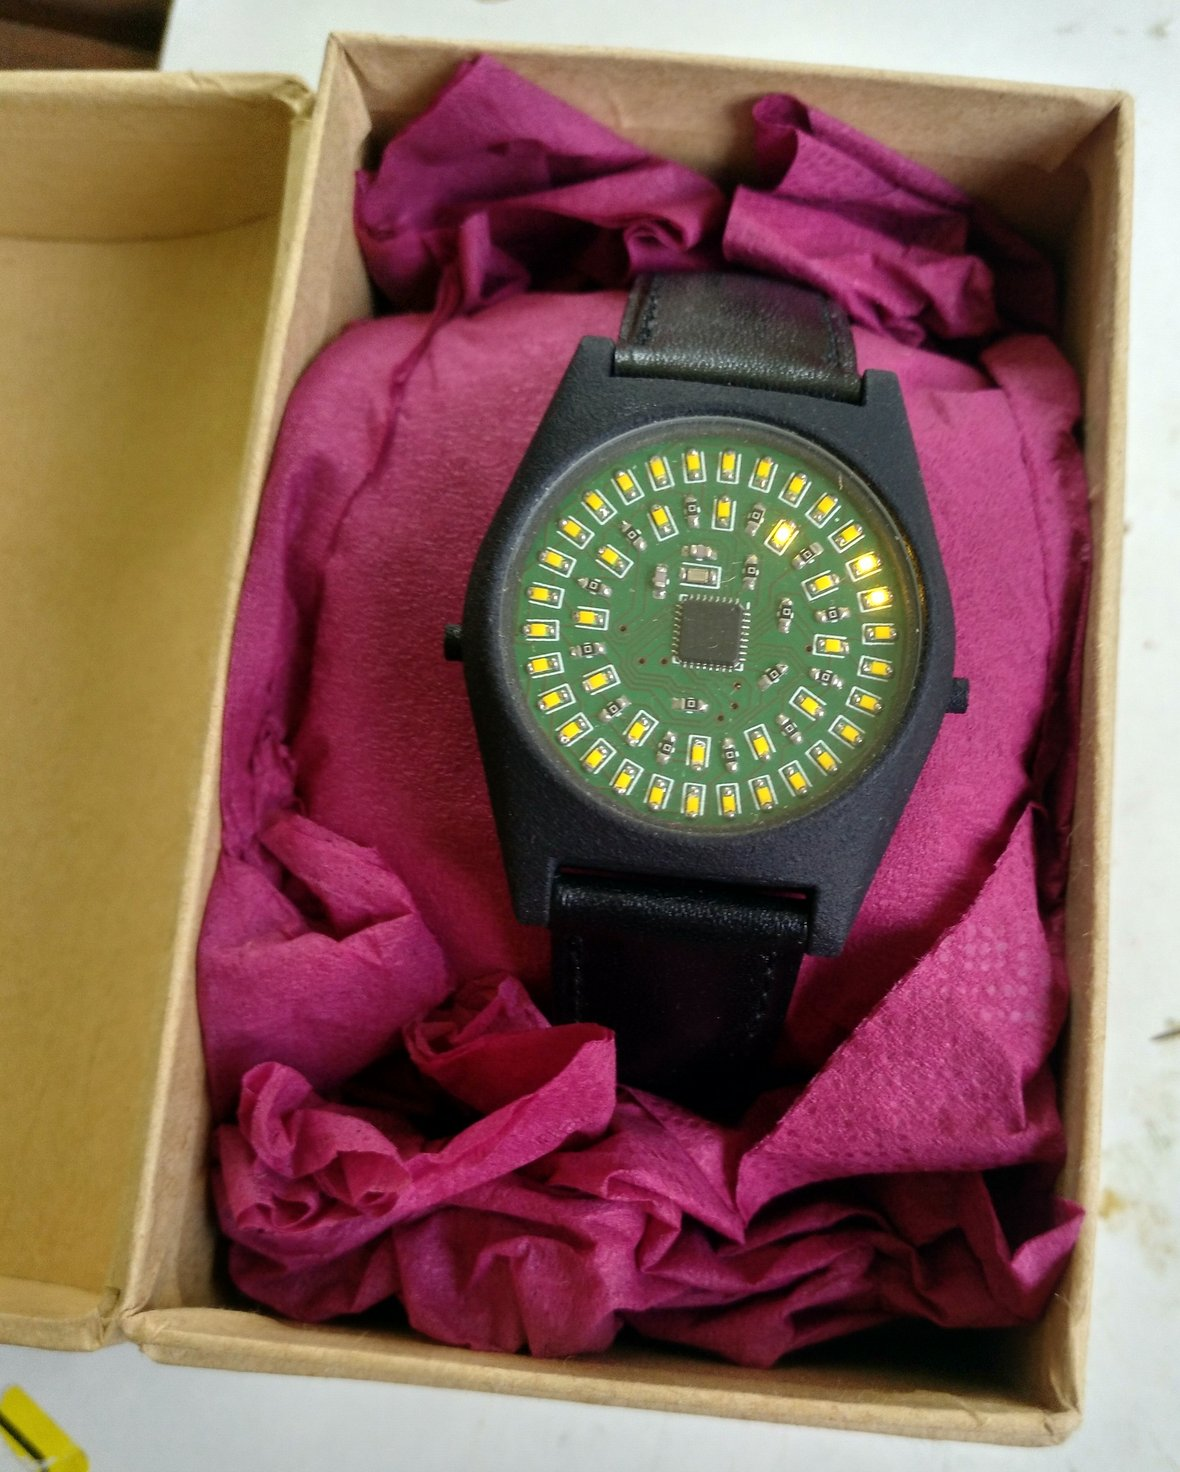
\includegraphics[width=0.7\textwidth]{../Pictures/AnalogWatch1.jpg}
\end{center}